\part{Systems of linear equations I - Introduction}
\section{Introduction}
\subsection*{General}
\begin{frame}[label=contentslin1]
  \frametitle{Today's outline}
  \mode<beamer>{
    \only<1>{\tableofcontents}
  }
  \only<2>{\tableofcontents[currentsection,currentsubsection]}
\end{frame}

\begin{frame}
  \frametitle{Overview}
  \begin{block}{Goals}
    \begin{itemize}
      \item Different ways of looking at a system of linear equations
      \item Determination of the inverse, determinant and the rank of a matrix
      \item The existence of a solution to a set of linear equations
  \end{itemize}
  \end{block}
\end{frame}
% 
\subsection*{Linear systems}

{\nologo
  \frame{\frametitle{Different views of linear systems}
    \begin{columns}
      \column{0.4\textwidth}
    \begin{itemize}
      \vskip-1ex
      \item Separate equations:\vspace{-1em}\begin{align*}
        x + y +  z &= 4 \\
        2x + y + 3z &= 7 \\
        3x + y + 6z &= 5
      \end{align*} \pause
      \item Matrix mapping $Mx=b$:\vspace{-1ex} \[ 
        \begin{bmatrix}
    1 & 1 & 1\\ 
    2 & 1 & 3\\ 
    3 & 1 & 6
        \end{bmatrix}
        \begin{bmatrix}
    x \\
    y \\
    z 
        \end{bmatrix} = 
        \begin{bmatrix}
    4 \\
    7 \\
    5 
        \end{bmatrix} 
        \]
        \pause
      \item Linear combination:\vspace{-1ex} \[ 
        x \begin{bmatrix}
    1\\
    2\\
    3
    \end{bmatrix} +
        y \begin{bmatrix}
    1\\
    1\\
    1
    \end{bmatrix} +
        z \begin{bmatrix}
    1\\
    3\\
    6
    \end{bmatrix} =
    \begin{bmatrix}
    4\\
    7\\
    5
        \end{bmatrix} 
      \]
      \end{itemize}
      \column{0.6\textwidth}
      \pause
      \centering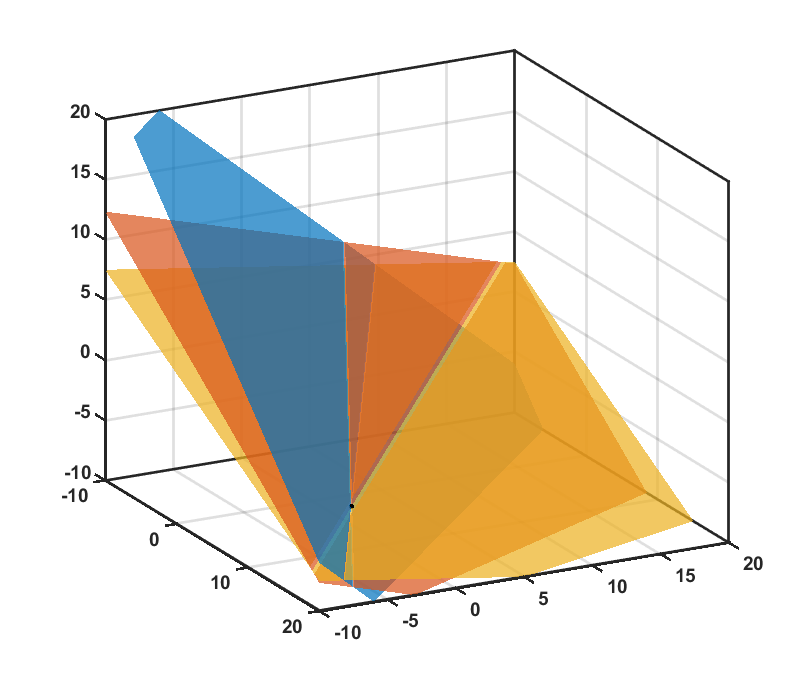
\includegraphics[width=\columnwidth]{planes_xing.png}
    \end{columns}
  }
}

\section{Matrix inversion}
\subsection*{Inverse}
\againframe<2>{contentslin1}

\frame{
  \frametitle{Inverse of a matrix}
  \begin{itemize}
    \item The inverse $M^{-1}$ is defined such that:
   \[ MM^{-1} = I \quad{} \text{and} \quad{} M^{-1}M=I\]
   \item Use the inverse to solve a set of linear equations:
   \begin{align*}
    M\vec{x} &= \vec{b} \\
    M^{-1}M\vec{x} &= M^{-1}\vec{b} \\
    I\vec{x} &= M^{-1}\vec{b} \\
    \vec{x} &= M^{-1}\vec{b}
   \end{align*}
  \end{itemize}
}
% 
\frame{\frametitle{How to calculate the inverse?}
  \begin{itemize}
    \item The inverse of an $N \times N$ matrix can be calculated using the co-factors of each element of the matrix:
    \[
      M^{-1} = \frac{1}{\det{M}}
      \begin{bmatrix}
      C_{11} &C_{12} &C_{13} \\
      C_{21} &C_{22} &C_{23} \\
      C_{31} &C_{32} &C_{33} \\
      \end{bmatrix}^T
    \]
    \item $\det{M}$ is the \emph{determinant} of matrix $M$.
    \item $C_{ij}$ is the \emph{co-factor} of the $ij^\text{th}$ element in $M$.
    \item $M^T$ indicates the transpose of a matrix $M$
  \end{itemize}
}

\begin{frame}[fragile]
\frametitle{Computing the co-factors}
  Consider the following example matrix:
  $ M =
    \begin{bmatrix}
      1 & 1 & 1\\ 
      2 & 1 & 3\\ 
      3 & 1 & 6
    \end{bmatrix} 
  $\\ \vskip1em \pause
  A co-factor (e.g. $C_{11}$) is the \tikzmarkin[txt=style green]{det1}determinant of the elements left over\tikzmarkend{det1} when you cover up the row and column of the \tikzmarkin[txt=style cyan]{cof}element in question\tikzmarkend{cof}, \tikzmarkin[txt=style orange]{pm1}multiplied by $\pm 1$\tikzmarkend{pm1}, depending on the position. \vskip1em
  \begin{columns}
    \column{0.25\textwidth}
      \begin{equation*}
      \left[\begin{array}{ccc}
	\tikzmarkin[mat=style cyan]{col 1} 1 \tikzmarkend{col 1} &  \times & \times \\
	\times  & \tikzmarkin[mat=style green]{col 2} 1 & 3 \\
	\times  &  1   &  6 \tikzmarkend{col 2}\\
	\end{array}\right]
      \end{equation*}\pause
    \column{0.25\textwidth}
      \begin{equation*}
      \left[\begin{array}{ccc}
	\tikzmarkin[mat2=style orange]{pm} + \tikzmarkend{pm} &  - & + \\
	- & + & - \\
	+ & - & +\\
	\end{array}\right]
      \end{equation*}\pause
      \column{0.5\textwidth}
      \[ \begin{split}
C_{11} &= \tikzmarkin[mat2=style orange]{pm3}+1\tikzmarkend{pm3}\ \cdot\ \det{\begin{array}{cc}\tikzmarkin[mat=style green]{det2} 1 & 3 \\ 1 & 6\tikzmarkend{det2}\end{array}} \\
&= 6 \times 1 - 3 \times 1 = 3
\end{split}
\]
  \end{columns}
\end{frame}

\frame{\frametitle{Computing the co-factors}
    Back to our example:
    \[
      M^{-1} = \begin{bmatrix}
      1 & 1 & 1 \\
      2 & 1 & 3 \\
      3 & 1 & 6 \\
    \end{bmatrix}^{-1} = 
      \frac{1}{\det{M}}
      \begin{bmatrix}
      3 & -3 & -1 \\
      -5&  3 &  2 \\
      2 & -1 & -1 \\
      \end{bmatrix}^T
    \]\pause
    \begin{itemize}
      \item The determinant is very important
      \item If $\det{M}=0$, the inverse does not exist (singular matrix)
      \begin{itemize}
        \item E.g. when a row contains only zeros, or when a row is a scalar multiple of another row.
      \end{itemize}
    \end{itemize}
}

\frame{\frametitle{Calculating the determinant}
    Compute the determinant by multiplication of each element on a row (or column) by its cofactor and adding the results:
    \[
    \det{\begin{bmatrix}
      \ \tikzmarkin[mat=style green]{horizontal}1 & 1 & 1 \tikzmarkend{horizontal}\\
      2 & 1 & 3 \\
      3 & 1 & 6 \ \end{bmatrix}} = +\det{\begin{bmatrix}1&3\\1&6\end{bmatrix}} - \det{\begin{bmatrix}2&3\\3&6\end{bmatrix}} + \det{\begin{bmatrix}2&1\\3&1\end{bmatrix}} = -1
    \]
    \pause
    \[
    \det{\begin{bmatrix}
      \ 1 & 1 & \tikzmarkin[mat=style green]{vertical}1 \\
      2 & 1 & 3 \\
      3 & 1 & 6\tikzmarkend{vertical}\ \end{bmatrix}} = +\det{\begin{bmatrix}2&1\\3&1\end{bmatrix}} - 3\det{\begin{bmatrix}1&1\\3&1\end{bmatrix}} + 6\det{\begin{bmatrix}1&1\\2&1\end{bmatrix}} = -1
    \]
}

\section{Solving a linear system}
\subsection*{Solving}
\againframe<2>{contentslin1}

\frame{\frametitle{Solving a linear system}
  \begin{itemize}
    \item Our example:
   \[ 
      \begin{bmatrix}
	1 & 1 & 1\\ 
	2 & 1 & 3\\ 
	3 & 1 & 6
      \end{bmatrix}
      \begin{bmatrix}
	x \\
	y \\
	z 
      \end{bmatrix} = 
      \begin{bmatrix}
	4 \\
	7 \\
	5 
      \end{bmatrix} 
      \]\pause
    \item The solution is:
    \[
    \begin{bmatrix}x \\ y \\ z\end{bmatrix} = M^{-1}b= \frac{1}{-1}
    \begin{bmatrix}
      3 & -5 & 2 \\
      -3&  3 & -1 \\
      -1 & 2 & -1 \\
    \end{bmatrix} \begin{bmatrix}4 \\ 7 \\ 5\end{bmatrix} = \frac{1}{-1}\begin{bmatrix}-13 \\ 4 \\ 5\end{bmatrix} = \begin{bmatrix}13 \\ -4 \\ -5\end{bmatrix}
    \]\pause
    \item The inverse exists, because $\det{M}=-1$.
  \end{itemize}
}

\begin{frame}[fragile]
  \frametitle{Solving a linear system in Python using the inverse}
  \begin{itemize}
    \item Set the scene by importing the right modules:
    \begin{lstlisting}
import numpy as np
import numpy.linalg as npla # scipy.linalg also works!
    \end{lstlisting}
    \item Create the matrix $A$ (explicit indication of datatype):
    \begin{lstlisting}
A = np.array([[1,1,1],[2,1,3],[3,1,6]],dtype=np.float64)
    \end{lstlisting}\pause
    \item Create solution vector (column vector):
    \begin{lstlisting}
b = np.array([[4.,7.,5.]]).T # Check b.shape!
    \end{lstlisting}\pause
    \item Get the matrix inverse; we use the linalg submodule
    \begin{lstlisting}
Ainv = npla.inv(A)
    \end{lstlisting}\pause
    \item Compute the solution:  %
    \begin{multicols}{2}
\begin{lstlisting}[linewidth=0.45\textwidth]
solution = Ainv.dot(b)
print(f'The solution is:\n {solution}')
\end{lstlisting}      \break
\begin{lstlisting}[style=output,linewidth=0.45\textwidth]
The solution is:
[[13.]
[-4.]
[-5.]]
\end{lstlisting}
\end{multicols}
  \end{itemize}
\end{frame}

\begin{frame}[fragile]
  \frametitle{Solving a linear system in Python: recommended approach}
  \begin{columns}
    \column{0.5\textwidth}
      NumPy approach
      \begin{lstlisting}
# solve_system_np.py
import numpy as np
import numpy.linalg as npla

A = np.array([[1.,1.,1.],[2.,1.,3.],[3.,1.,6.]])
b = np.array([[4.,7.,5.]]).T
x = npla.solve(A,b)
print(f'Solution using np linalg:\n {x}')
        \end{lstlisting}
        \begin{lstlisting}[style=output]
Solution using np linalg:
[[13.]
[-4.]
[-5.]]
        \end{lstlisting}
    \column{0.5\textwidth}
    SciPy approach
    \begin{lstlisting}
# solve_system_sp.py
import numpy as np
import scipy.linalg as spla

A = np.array([[1.,1.,1.],[2.,1.,3.],[3.,1.,6.]])
b = np.array([[4.,7.,5.]]).T
x = spla.solve(A,b)
print(f'Solution using sp linalg:\n {x}')      
      \end{lstlisting}
      \begin{lstlisting}[style=output]
Solution using sp linalg:
[[13.]
[-4.]
[-5.]]
    \end{lstlisting}
  \end{columns}
  Paraphrased from the NumPy manual:
  There is overlap in the functionality provided by the SciPy and NumPy submodules. SciPy contains functions not found in \lstinline$numpy.linalg$. Some functions that exist in both have augmented functionality in \lstinline$scipy.linalg$. Some functions in NumPy, however, have more flexible broadcasting options.
\end{frame}
{\nologo
\begin{frame}<handout:0|beamer:1->[fragile]
  \frametitle{Exercise: performance of inverse computation}
  Create a script that generates matrices with random elements of various sizes $N\times N$ (e.g. values of $N\in\left\{10,20,50,100,200,\ldots,5000,10000\right\}$). Compute the inverse of each matrix, and use \lstinline$tic$ and \lstinline$toc$ to see the computing time for each inversion. Plot the time as a function of the matrix size $N$. \pause
    \begin{lstlisting}
import numpy as np
import scipy.linalg as spla
from time import time
import matplotlib.pyplot as plt

matrix_sizes = list(range(10,100,10)) + list(range(100,1100,100)) + list(range(2000,6000,1000)) + [10000]

for size in matrix_sizes: (*@ \pause @*)
    print(f'Currently processing matrix size: {size}x{size}')
    random_matrix = np.random.random((size,size)) (*@ \pause @*)
    start_time = time()
    spla.inv(random_matrix)
    total_time = time() - start_time
    time_to_inv.append(total_time)
    (*@ \pause @*)
plt.loglog(matrix_sizes,time_to_inv, 'r-x')
plt.xlabel('Matrix size')
plt.ylabel('Time to invert [s]')
plt.show()
  \end{lstlisting}
\end{frame}
}

\begin{frame}<beamer:0|handout:1>[fragile]
  \frametitle{Exercise: performance of inverse computation}
  Create a script that generates matrices with random elements of various sizes $N\times N$ (e.g. values of $N\in\left\{10,20,50,100,200,\ldots,5000,10000\right\}$). Compute the inverse of each matrix, and use \lstinline$tic$ and \lstinline$toc$ to see the computing time for each inversion. Plot the time as a function of the matrix size $N$.
  \vskip2em
  \begin{hints}
  Hints:
  \begin{itemize}
      \item Create an array that contains the sizes of the systems $n$
      \item Loop over the array elements to:
      \begin{itemize}
          \item Create a random matrix of size $n\times n$
          \item Perform the matrix inversion
          \item Record the time required
      \end{itemize}
      \item Plot the time required for inversion vs size of the system on a double-log scale
  \end{itemize}
  \end{hints}
\end{frame}

\begin{frame}[fragile]
  \frametitle{Exercise: sample results}
  Each computer produces slightly different results because of background tasks, different matrices, etc. This is especially noticable for small systems.
  \begin{center}
  \begin{tikzpicture}
    \begin{loglogaxis}[
      xlabel={$N$},
      ylabel={Time [s]},
%       grid = major,
      width=0.6\textwidth, height=5.5cm]
     \addplot[graph,draw=tuered,thick,mark = x] table [y index={1}] {data/tictocINV.dat};
     \addplot [black,very thick] table {
	900 0.065
	11000 64.87
      } coordinate [pos=0.15] (A) % save two points on the regression line for drawing the slope triangle
        coordinate [pos=0.85] (B);
	\draw[thick] (A) -| (B)  % draw the opposite and adjacent sides of the triangle
        node [pos=0.25, anchor=north] {1} % label the horizontal line
        node [pos=0.75,anchor=west] {3};
     \end{loglogaxis}
  \end{tikzpicture}
  \end{center}
  \vskip-1em
  \tikzmarkin[txt=style white]{complexity}The time increases by 3 orders of magnitude, for every magnitude in $N$. The \emph{computational complexity} of matrix inversion scales with $\mathcal{O}(N^3)$!\tikzmarkend{complexity}
\end{frame}

\begin{frame}[fragile]
  \frametitle{Solving a linear system in Excel using the inverse}\vspace{-1em}
  \[
   Ax=b \qquad \begin{bmatrix}1&1&1\\2&1&3\\3&1&6\end{bmatrix}\begin{bmatrix}x_1\\x_2\\x_3\end{bmatrix}=\begin{bmatrix}4\\7\\5\end{bmatrix}
  \]\vspace{-1em}
  \begin{itemize}
    \item Create matrix \ \tikzmarkin[mat=style green]{A}$A$\tikzmarkend{A} \ in $3\times 3$ cells
    \item Create right hand side vector \ \tikzmarkin[mat=style cyan]{b}$b$\tikzmarkend{b} \ in 3 vertical cells\pause
    \item Compute the inverse \ \tikzmarkin[mat=style orange]{I}$I$\tikzmarkend{I} \ :
    \begin{itemize}
      \item Select an empty area of $3 \times 3$ cells
      \item Type \lstinline$=MINVERSE($
      \tikzmarkin[txt=style green]{A2}\lstinline$B2:D4$\tikzmarkend{A2}
      \lstinline$)$ (In Dutch Excel: \lstinline$INVERSEMAT$)
      \item Close with Ctrl+Shift+Enter
    \end{itemize}\pause
    \item Solution:
    \begin{itemize}
      \item Select 3 vertical cells
      \item Type \lstinline$=MMULT($
      % First part, contains the inverse
      \tikzmarkin[txt=style orange]{I2}\lstinline$H2:J4$\tikzmarkend{I2}
      % Semicolon
      \lstinline$;$
      % Second part, contains the RHS
      \tikzmarkin[txt=style cyan]{b2}\lstinline$B6:B8$\tikzmarkend{b2}
      % Finish the command
      \lstinline$)$ (In Dutch Excel: \lstinline$PRODUCTMAT$. The semicolon may be a comma.)
      \item Close with Ctrl+Shift+Enter
    \end{itemize}    
  \end{itemize}
\end{frame}


\section{Towards larger systems}
\subsection*{Matrix tricks}
\againframe<2>{contentslin1}

\begin{frame}[fragile]
  \frametitle{Towards larger systems}
  \tikz{\node[emphblock,text width=\textwidth] {Computation of determinants and inverses of large matrices in this way is too difficult (slow), so we need other methods to solve large linear systems!};}
\end{frame}

\begin{frame}[fragile]
  \frametitle{Towards larger systems}
  \begin{itemize}
    \item Determinant of upper triangular matrix:
    \[
    \det{M_\text{tri}} = \prod_{i=1}^n a_{ii} \qquad M=\begin{bmatrix}
5 & 3 & 2 \\ 
0 & 9 & 1 \\
0 & 0 & 1
\end{bmatrix} \Rightarrow \det{M} = 5 \times 9 \times 1 = 45
    \]
  \item Matrix multiplication:
  \[
  \det{AM}=\det{A}\times\det{M}
  \]
  \item When $A$ is an identity matrix ($\det{A}=1$):
  \[
   \det{AM}=\det{A}\times\det{M} = 1\times\det{M}
  \]
  \item With rules like this, we can use row-operations so that we can compute the determinant more cheaply.
  \end{itemize}
\end{frame}

\subsection*{Rank}
\begin{frame}[fragile]
  \frametitle{Solutions of linear systems}
 Rank of a matrix: the number of linearly independent columns (columns that can not be expressed as a linear combination of the other columns) of a matrix.
 \vskip1em
 \begin{columns}
  \column{0.5\textwidth}
  \[
   M = \begin{bmatrix}
        5 & 3 & 2 \\
        0 & 9 & 1 \\
        0 & 0 & 1
       \end{bmatrix}
  \]
  \begin{itemize}
   \item 3 independent columns
   \item In Matlab:
   \begin{lstlisting}
>> rank(M)
   \end{lstlisting}
  \end{itemize}
  \column{0.5\textwidth}
    \[
   M = \left[\begin{array}{cccc}
        \tikzmarkin[mat=style green]{c1}1 & \tikzmarkin[mat=style yellow]{c2}2 & \tikzmarkin[mat=style cyan]{c3}1 & \tikzmarkin[mat=style orange]{c4}0 \\
        0 & 0 & 1 & 1 \\
        0\tikzmarkend{c1} & 0\tikzmarkend{c2} & 0\tikzmarkend{c3} & 0\tikzmarkend{c4}
       \end{array}\right]
  \]
  \begin{itemize}
   \item \tikzmarkin[txt=style yellow]{c22}col 2\tikzmarkend{c22} $= 2 \times$ \tikzmarkin[txt=style green]{c12}col 1\tikzmarkend{c12}
   \item \tikzmarkin[txt=style orange]{c42}col 4\tikzmarkend{c42} $=$ \tikzmarkin[txt=style cyan]{c32}col 3\tikzmarkend{c32} $-$ \tikzmarkin[txt=style green]{c13}col 1\tikzmarkend{c13}
   \item 2 independent columns: rank = 2
  \end{itemize}
 \end{columns}
\end{frame}

\begin{frame}[fragile]
  \frametitle{Solutions of linear systems}
  The solution of a system of linear equations may or may not exist, and it may or may not be unique. Existence of solutions can be determined by comparing the rank of the Matrix $M$ with the rank of the augmented matrix $M_a$:
  \begin{lstlisting}
>> rank(A)
>> rank([A b])
  \end{lstlisting}
  Our system: $Mx = b$\\
  \[ 
    M = \begin{bmatrix}
    M_{11} & M_{12} & M_{13}\\ 
    M_{21} & M_{22} & M_{23}\\ 
    M_{31} & M_{32} & M_{33}
    \end{bmatrix} \text{,} b=\begin{bmatrix}b_1\\b_2\\b_3  \end{bmatrix} \Rightarrow 
    M_a =     \begin{bmatrix}
    M_{11} & M_{12} & M_{13} & b_1\\ 
    M_{21} & M_{22} & M_{23} & b_2\\ 
    M_{31} & M_{32} & M_{33} & b_3
    \end{bmatrix}
  \]
\end{frame}

\begin{frame}
 \frametitle{Existence of solutions for linear systems}
  For a matrix $M$ of size $n \times n$, and augmented matrix $M_a$:
 \begin{columns}
  \column{0.5\textwidth}
 \begin{itemize}
   \item $\text{Rank}(M) = n$:\\ Unique solution
 \end{itemize}
  \column{0.5\textwidth}
   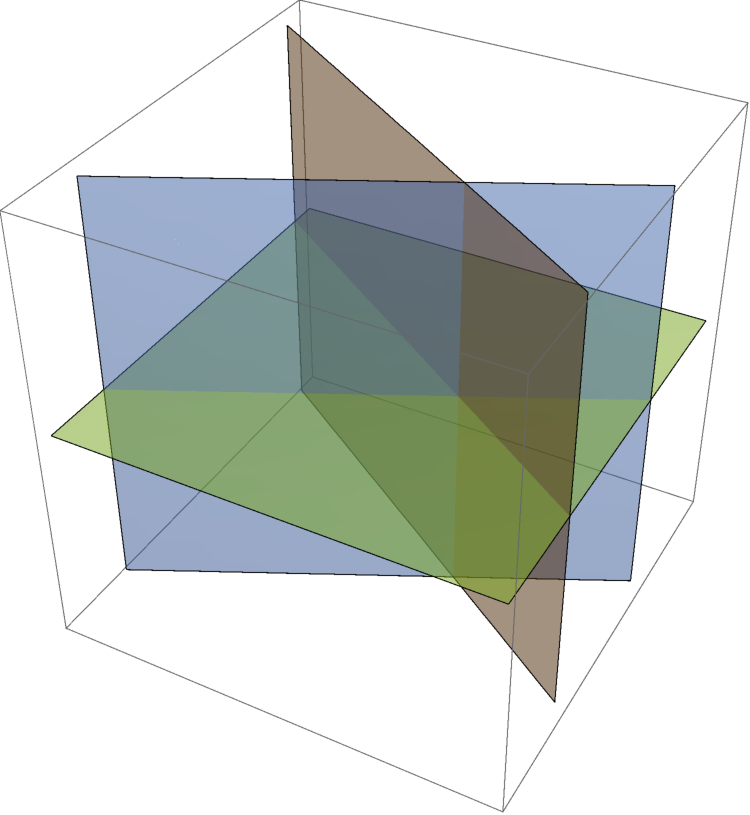
\includegraphics[width=0.3\columnwidth]{Rank_1-solution}
 \end{columns}
 \pause
  \begin{columns}
  \column{0.5\textwidth}
 \begin{itemize}
   \item $\text{Rank}(M) = \text{Rank}(M_a) < n$:\\ Infinite number of solutions
 \end{itemize}
  \column{0.5\textwidth}
   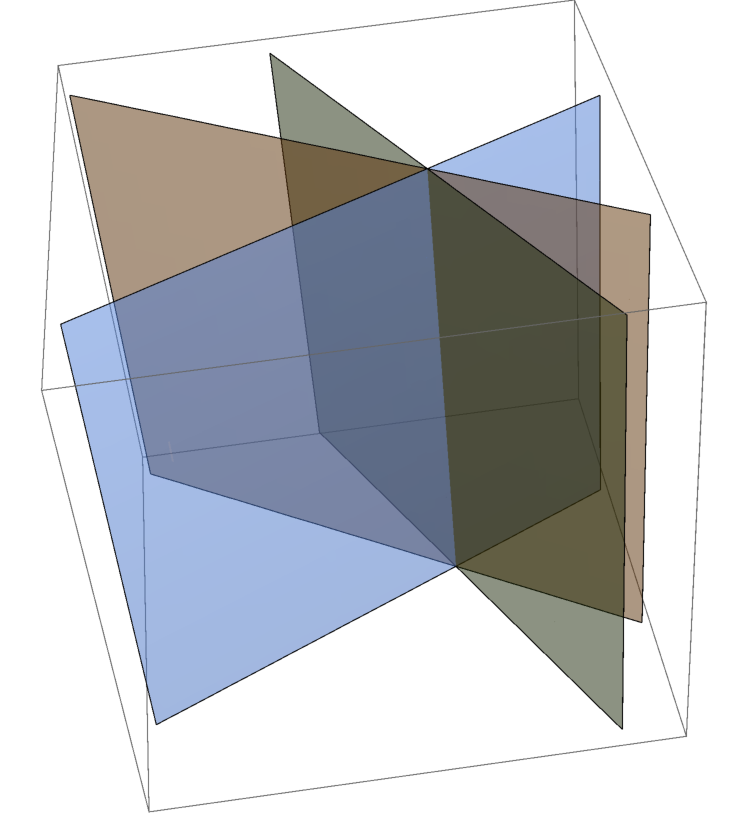
\includegraphics[width=0.3\columnwidth]{Rank_Inf-solutions}
 \end{columns}
 \pause
  \begin{columns}
  \column{0.5\textwidth}
 \begin{itemize}
   \item $\text{Rank}(M) < n$, $\text{Rank}(M) < \text{Rank}(M_a)$:\\ No solutions
 \end{itemize}
  \column{0.5\textwidth}
   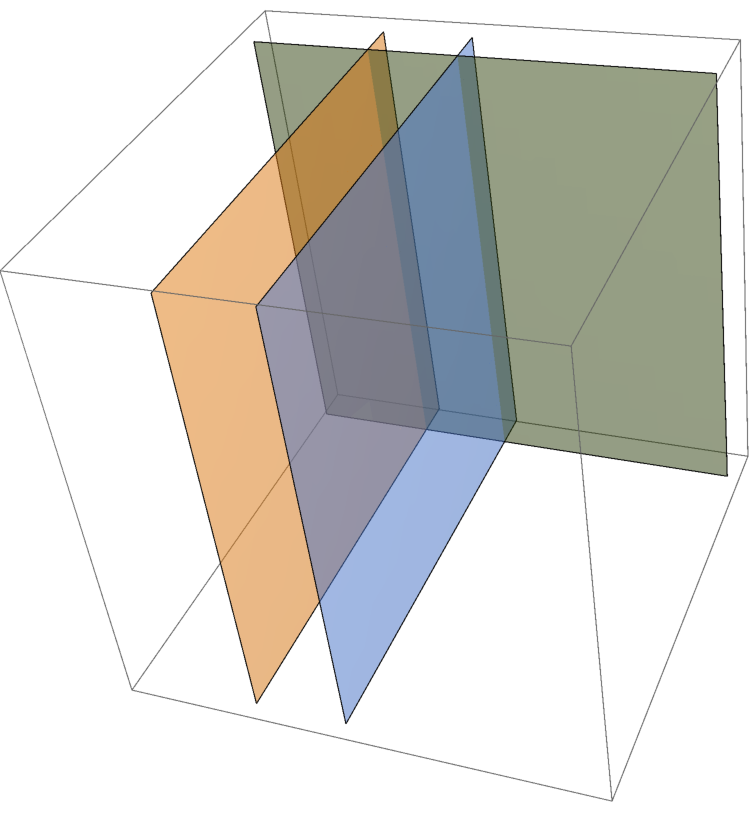
\includegraphics[width=0.3\columnwidth]{Rank_No-solutions1} \ \ 
   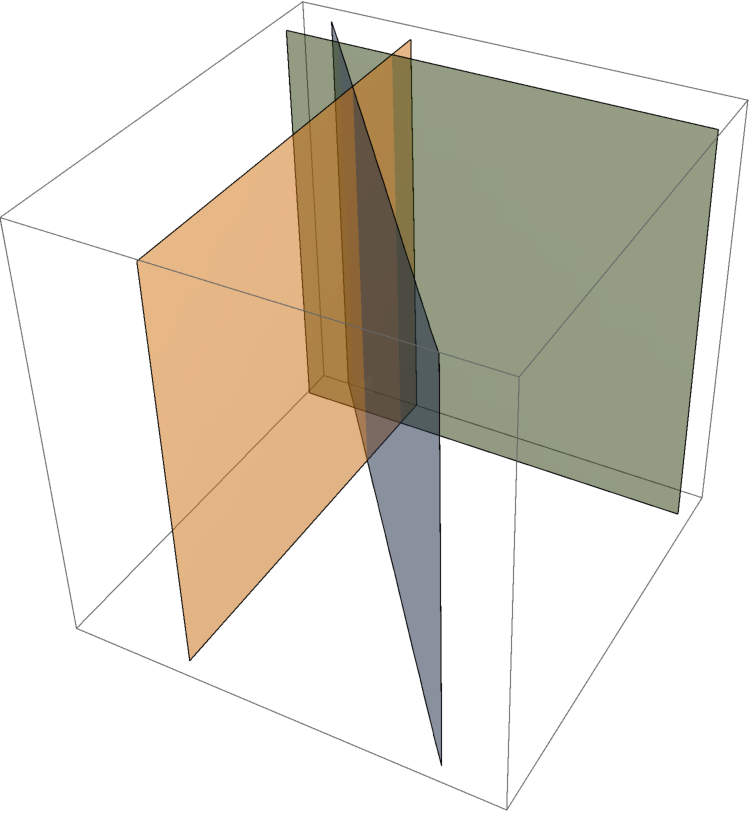
\includegraphics[width=0.3\columnwidth]{Rank_No-solutions2}
 \end{columns}
\end{frame}
 
\begin{frame}[fragile]
  \frametitle{Two examples}
  \[
    M=
    \begin{bmatrix}
      1 & 1 & 2\\
      0 & 3 & 1\\
      0 & 0 & 2
    \end{bmatrix}\quad
    b=
    \begin{bmatrix}
      17\\11\\4
    \end{bmatrix}
    \Rightarrow
    M_a=
    \begin{bmatrix}
      1 & 1 & 2 & 17\\
      0 & 3 & 1 & 11\\
      0 & 0 & 2 & 4
    \end{bmatrix}
  \]
  $\rank(M)=3=n \Rightarrow $ Unique solution \pause \\ \vfill
    \[
    M=
    \begin{bmatrix}
      1 & 1 & 2\\
      0 & 3 & 1\\
      0 & 0 & 0
    \end{bmatrix}\quad
    b=
    \begin{bmatrix}
      17\\11\\0
    \end{bmatrix}
    \Rightarrow
    M_a=
    \begin{bmatrix}
      1 & 1 & 2 & 17\\
      0 & 3 & 1 & 11\\
      0 & 0 & 0 & 0
    \end{bmatrix}
  \]
  $\rank(M)=\rank(M_a)=2<n \Rightarrow $ Infinite number of solutions
\end{frame} 

\section{Summary}
\subsection*{Summary}
\againframe<2>{contentslin1}

\begin{frame}[fragile]
  \frametitle{Summary}
  \begin{itemize}
    \item Linear equations can be written as matrices
    \item Using the inverse, the solution can be determined
    \begin{itemize}
      \item Inverse via cofactors
      \item Inverse and solution in Matlab
      \item Inverse and solution in Excel
    \end{itemize}
    \item Introduced the concept of computational complexity: matrix inversion scales with $N^3$
    \item A solution depends on the rank of a matrix
  \end{itemize}
\end{frame}